\documentclass{article}
\usepackage{graphicx} % Required for inserting images
\usepackage{amsfonts}
\usepackage{amsmath}
\usepackage[ruled,vlined]{algorithm2e}
\usepackage{graphicx}
\usepackage{hyperref}

\graphicspath{ {./images/} }


\title{Analisi di due campioni bi-variati}
\author{Enrico Cotti Cottini}
\date{March 2024}

\begin{document}

\maketitle

\section{Introduction}

Sia $\{x_i , y_i\}_i\in\{1,...,n\}$ un campione bi-variato di numerosità n.
\newline
Poniamo:
\[
    \phi(a,b)=\sum_{i=1}^{n}(y_i-(a\cdot x_i+b))^2 , (a,b)\in \mathbb{R}^2
\]
Si scriva un programma che dato $\{x_i , y_i\}_i\in\{1,...,n\}$, calcoli un punto di minimo di $\phi$, cioè un punto $(a_*,b_*)\in \mathbb{R}^2$ tale che
\[
    \phi (a_*,b_*)=min\{\phi(a,b):a,b\in\mathbb{R}\}
\]
Si considerino poi i due campioni bi-variati (Tmn,Tmed) e (Tmin,Ptot) del file \textbf{Meteo\_Chioggia60.ods} e si crei, per ciascuno dei due campioni bi-variati, il corrispondente diagramma di dispersione col grafico della retta $t \mapsto a_* t+b_*$ determinata dal punto di minimo $(a_*,b_*)$ calcolato col programma.

Per la consegna servono:
\begin{itemize}
\item una giustificazione matematica della procedura utilizzata per il calcolo di un punto di minimo di $\phi$
\item lo pseudo-codice del programma e il codice commentato in un linguaggio
standard come C++ o Python;
\item i grafici dei due diagrammi di dispersione con le rette di regressione in
formato pdf e i valori numerici dei punti di minimo utilizzati.
\end{itemize}


\section{Analisi}
Il problema si riduce alla ricerca di una retta
\[
    Y = \beta + \alpha x,\ \alpha,\beta \in\mathbb{R}
\]
che approssimi i dati dei diagrammi di disperione dei campioni bi-variati $\{x_i , y_i\}_i\in\{1,...,n\}$.
\newline
La ricerca dei valori $(a_*,b_*)\in \mathbb{R}^2$ che minimizzano $\phi$ tale che
\[
    \phi (a_*,b_*)=min\{\phi(a,b):a,b\in\mathbb{R}\}
\]
per $ \phi$ la somma dei quadrati degli scarti tra le risposte stimate e reali 
\[
    \phi(a,b)=\sum_{i=1}^{n}(y_i-(a\cdot x_i+b))^2 , (a,b)\in \mathbb{R}^2
\]
Corrisponde al Metodo dei minimi quadrati.
\section{Metodo dei minimi quadrati}
il metodo dei minimi quadrati consiste nello scegliere come stimatori di $\alpha$ e $\beta$ i due valori $a$ e $b$ che minimizzano $\phi$.Per calcolarli, deriviamo $\phi$ rispetto ad $a$ e $b$: 
\[
    \frac{\partial \phi} {\partial a} = -2\sum_{i=1}^{n}x_i(y_i-b-a\cdot x_i)
\]
\[
    \frac{\partial \phi} {\partial b} = -2\sum_{i=1}^{n}(y_i-b-a\cdot x_i)
\]
Per cercare i punti critici di $\phi$, ed in particolare il minimo,occorre uguagliare a zero le due espressioni, ottenendo il sistema

\[
\begin{cases}
    \sum_{i=1}^{n}x_i y_i=b\sum_{i=1}^{n}x_i + a\sum_{i=1}^{n}x_i ^2 \\
    \sum_{i=1}^{n}y_i=nb+a\sum_{i=1}^{n}x_i         
\end{cases}\,
\]
Queste sone dette equazioni normali. Se si pone 

\[
    \overline{y}=\frac{1}{n}\sum_{i=1}^{n}y_i \hspace{40pt} e \hspace{40pt} \overline{x}=\frac{1}{n}\sum_{i=1}^{n}x_i
\]
la seconda equazione normale diventa 
\[
    b = \overline{y}-a\overline{x}
\]
sostituendo questa formula al posto di $b$ nella prima otteniamo
\[
    \sum_{i=1}^{n}x_i y_i=(\overline{y}-a\overline{x})n\overline{x}+a\sum_{i=1}^{n}x_i ^2
\]
ovvero
\[
    a(\sum_{i=1}^{n}x_i ^2 -n\overline{x}^2)=\sum_{i=1}^{n}x_i Y_i -n\overline{x}\overline{y}
\]
da cui si ricava che 
\[
    a = \frac{\sum_{i=1}^{n}x_i y_i -n\overline{x}\overline{y}}{\sum_{i=1}^{n}x_i ^2 -n\overline{x}^2}
\]
gli stimatori dei minimi quadradi di $\alpha$ e $\beta$ corrispondenti alle variabili $x_i$ e $y_i$, $i =1,2,...,n$ sono rispettivamente:
\[
    a = \frac{\sum_{i=1}^{n}x_i y_i -n\overline{x}\overline{y}}{\sum_{i=1}^{n}x_i ^2 -n\overline{x}^2}
\]
\[
    b = \overline{y}-a\overline{x}
\]
la retta $y = b + ax$ è la stima della retta di regressione, ovvero la retta che interpola meglio i dati.

\section{Pseudo-codice}

Il codice è stato scritto in Python 3.12.0 con ausilio delle librerie \textbf{Pandas Numpy matplotlib} istruzioni in \textbf{README.md}.
\newline
In Main.py è presente il codice per caricare il dataset di \textbf{Meteo\_Chioggia60.ods} e il codice per plottare i grafici.
\newline
Il codice Effettivo per calcolare i coefficenti della retta utilizzando il metodo dei minimi quadrati è presente in \textbf{Ols.py}.
lo speudocodice di \textbf{Ols.py} è:
\newline

\begin{algorithm}[H]
\SetAlgoLined
\KwIn{Array(di numpy) $x$ and $y$}
\KwOut{Coefficienti $m$ e $q$ per la retta di regressione ai minimi quadrati}
\BlankLine
$m = \frac{{\sum_{i=1}^{n} x_i y_i - n \cdot \text{average}(x) \cdot \text{average}(y)}}{{\sum_{i=1}^{n} x_i^2 - n \cdot \text{average}(x)^2}}$\;
$q = \text{average}(y) - m \cdot \text{average}(x)$\;
\BlankLine
\Return{$m$, $q$}\;
\caption{Regressione dei minimi quadrati}
\end{algorithm}
L' operazione di sommatoria $\sum$ e il calcolo della media campionaria $\overline{x}$ sono eseguite rispettivamente dalle funzioni \textbf{sum(x)} e \textbf{np.average(x)} quest'ultima funzione di utilità presente nella libreria Numpy
\newpage
\section{Risultati e Conclusioni}

\begin{figure}[htbp]
    \centering
    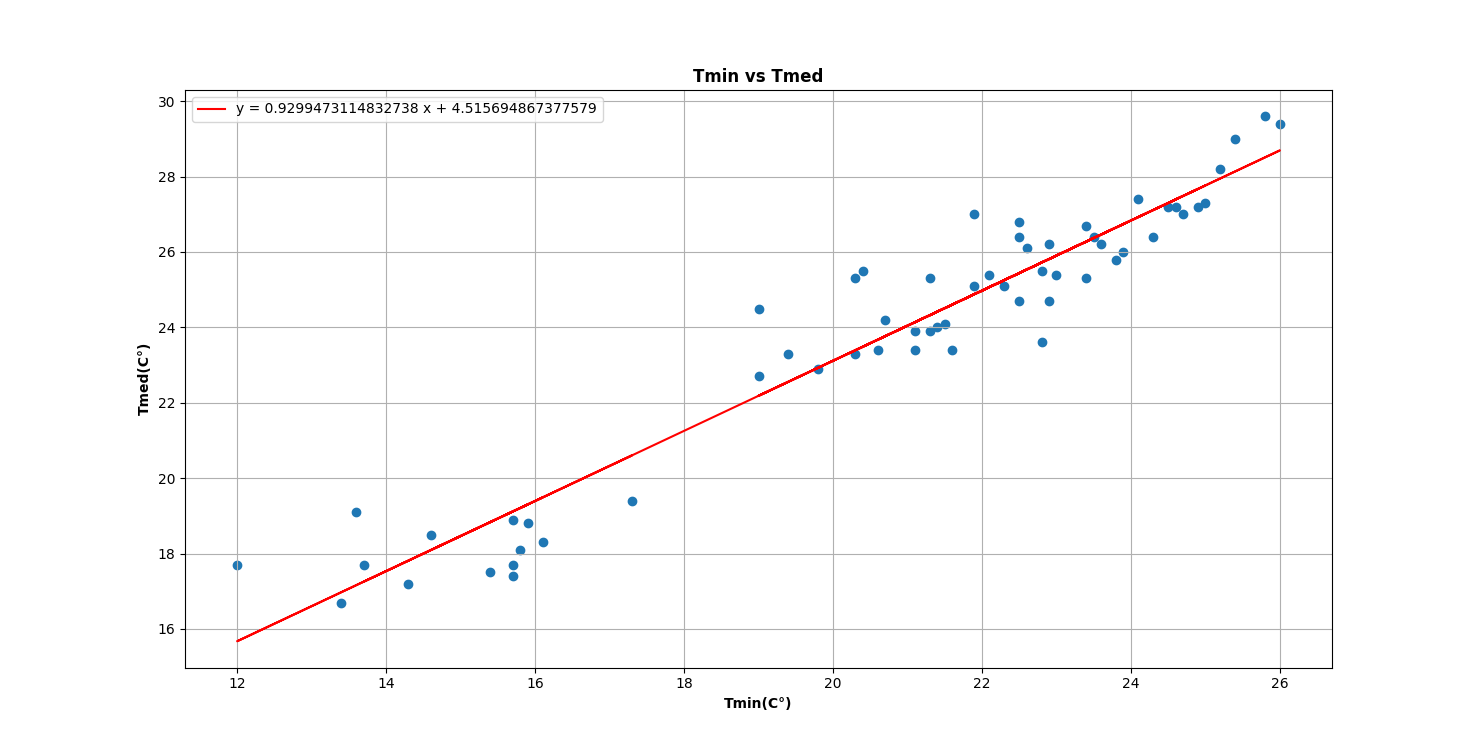
\includegraphics[width=0.9\textwidth]{images/Tmin_vs_Tmed.png}
    \caption{Tmin vs Tmed}
    \label{Tmin vs Tmed}
\end{figure}

La prima figura rappresenta il grafico di dispersione dei dati della temperatura Minima e Media in C°, nella Figura 1 possiamo Concludere che la regressione lineare sia uno strumento adatto per l'approssimazione dei dati.

\begin{figure}[htbp]
    \centering
    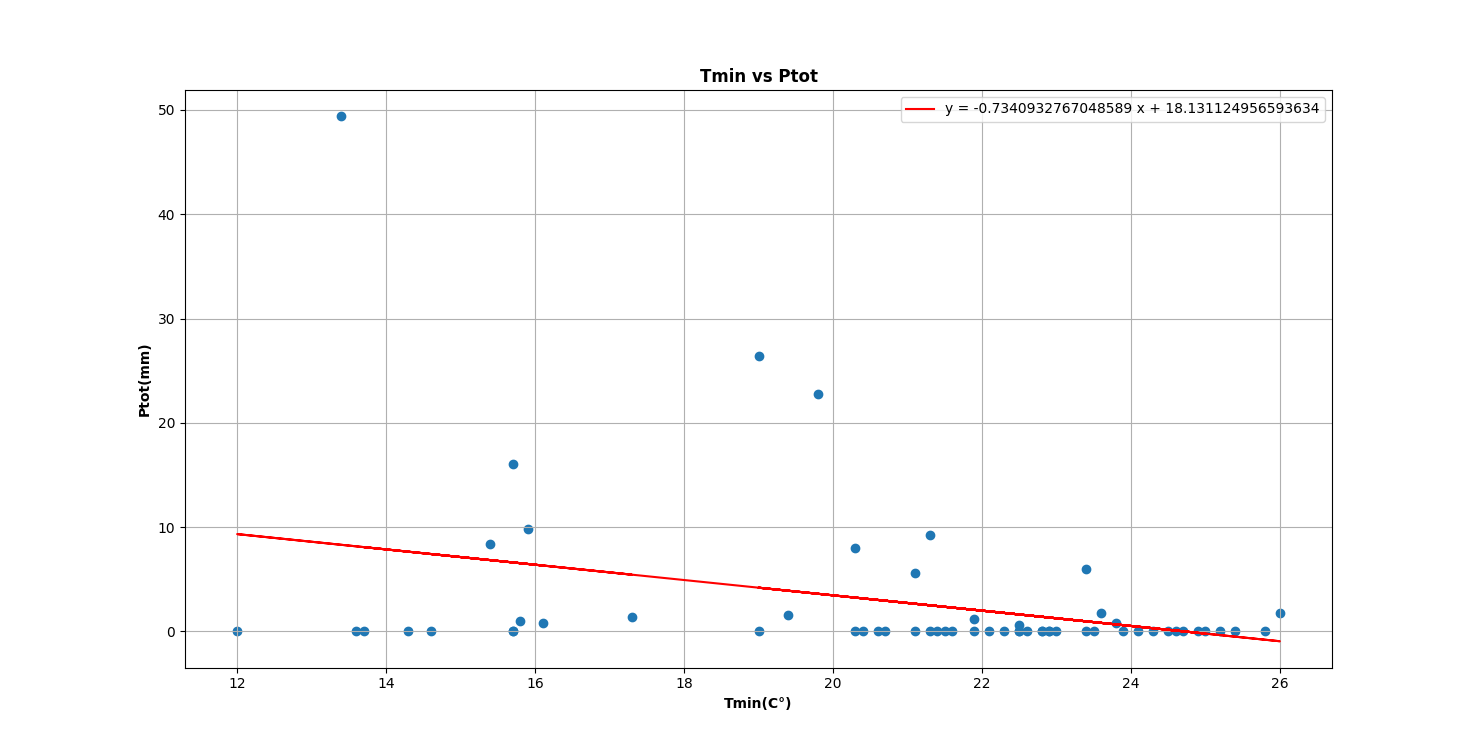
\includegraphics[width=0.9\textwidth]{images/Tmin_vs_Ptot.png}
    \caption{Tmin vs Ptot}
    \label{Tmin vs Ptot}
\end{figure}
La seconda figura rappresenta il grafico di dispersione dei dati della temperatura Media in C° e delle precipitazioni totali in mm, nella Figura 2 i dati sembrano essere più volatili rispetto alla prima, la regressione lineare potrebbe non essere il miglior metodo per approssimare i dati in questo caso.

\newpage

In conclusione analizzando per ognuno dei due campioni bi-variati del file \textbf{Meteo\_Chioggia60.ods}  è stato trovato il punto di minimo per cui 
\[
    \phi (a_*,b_*)=min\{\phi(a,b):a,b\in\mathbb{R}\}
\]
\newline
Nel \textbf{primo caso} i coeficienti trovati $m_*$ e $q_*$ (Coeficienti di regressione per\textbf{ Tmin vs Tmed}): 

\[
    \phi (m_1,q_1)=min\{\phi(m,q):m,q\in\mathbb{R}\}
\]
Che costruiscono la retta $y = q_1 + m_1 x$, Sono:

\[
    m_1 =  0.9299473114832738
\]
\[
    q_1 =  4.515694867377579
\]

Nel \textbf{secondo caso} i coeficienti trovati $m_*$ e $q_*$ (Coeficienti di regressione per\textbf{ Tmin vs Ptot}): 

\[
    \phi (m_2,q_2)=min\{\phi(m,q):m,q\in\mathbb{R}\}
\]
Che costruiscono la retta $y = q_2 + m_2 x$, Sono:

\[
    m_2 =  -0.7340932767048589 
\]
\[
    q_2 =  18.131124956593634
\]

\section{Interpretazione dei coefficienti di regressione}

Analizzando l'espressione dei coefficienti di regressione
\[
    a = \frac{\sum_{i=1}^{n}x_i y_i -n\overline{x}\overline{y}}{\sum_{i=1}^{n}x_i ^2 -n\overline{x}^2}
\]
\[
    b = \overline{y}-a\overline{x}
\]

In particolare $a$, Sommando e sottraendo $n\overline{xy}$ al numeratore e $n\overline{x}^2$ al denominatore

\[
    \frac{\sum_{i=1}^{n}x_i y_i -n\overline{x}\overline{y}-n\overline{x}\overline{y}+n\overline{x}\overline{y}}{\sum_{i=1}^{n}x_i ^2 -2n\overline{x}^2+n\overline{x}^2}
\]
Essendo $\overline{x}$ e $\overline{y}$ costanti e $n\overline{x}=\sum_{i=1}^{n}x_i$, $n\overline{y}=\sum_{i=1}^{n}y_i$

\[
    \frac{\sum_{i=1}^{n}x_i y_i -\sum_{i=1}^{n}x_i\overline{y}-\sum_{i=1}^{n}\overline{x}y_i+\sum_{i=1}^{n}\overline{x}\overline{y}}{\sum_{i=1}^{n}x_i ^2 -\sum_{i=1}^{n}2x_i\overline{x}+\sum_{i=1}^{n}\overline{x}^2}
\]
Quindi
\[
    \frac{\sum_{i=1}^{n}(x_i y_i -x_i\overline{y}-\overline{x}y_i+\overline{x}\overline{y})}{\sum_{i=1}^{n}(x_i ^2 -2x_i\overline{x}+\overline{x}^2)}
\]
Dunque otteniamo
\[
    a=\frac{\sum_{i=1}^{n}(x_i - \overline{x})(y_i - \overline{y})}{\sum_{i=1}^{n}(x_i - \overline{x})^2}
\]
dati covarianza e varianza campionaria, $COV_x_y$ e $S_x$, moltiplico e divido $\frac{1}{n-1}$

\[
    COV_x_y = \frac{1}{n-1}\sum_{i=1}^{n}(x_i - \overline{x})(y_i - \overline{y})
\]

\[
    S_x=\frac{1}{n-1}\sum_{i=1}^{n}(x_i - \overline{x})^2
\]

\[
    a=\frac{\frac{1}{n-1}\sum_{i=1}^{n}(x_i - \overline{x})(y_i - \overline{y})}{\frac{1}{n-1}\sum_{i=1}^{n}(x_i - \overline{x})^2}=\frac{COV_x_y}{S_x}
\]

Quindi a e b i coefficienti di regressione sono dipendenti dipendenti da $COV_x_y$ e $S_x$,in particolare $COV_x_y$ sceglie il segno del coefficiente angolare della retta, se i dati di y hanno lo stesso valore la retta ha coeficiente 0 e rappresenta una costante, mentre se i dati di x tendono tutti lo stesso valore avviene un fenomeno chiamato \textbf{Collinearità} nella quale $\frac{COV_x_y}{S_x}\longrightarrow\frac{0}{0}$  e le rette assumono forme imprecise.


\section{Bibliografia}

\begin{itemize}
    \item \href{https://en.wikipedia.org/wiki/Linear_regression#Least-squares_estimation_and_related_techniques}{https://en.wikipedia.org/wiki/Linear_regression#Least-squares_estimation_and_related_techniques}
    \item Ross - Probabilità e statistica per l'ingegneria e le scienze Capitolo 9
    
\end{itemize}




\end{document}

